\chapter{Robot Dynamic}
\label{sec:robotdynamic}

In this appendix, the nomenclature and equations used in this thesis are presented.

\section{Equations of motions}
\label{sec:eom}

The general form of the equations of motion of robotic system (interconnected rigid body driven by actuators) are:

\begin{align}
H(\vec{q}) \vec{\ddot{q}} + C(\vec{q},\vec{\dot{q}}) \vec{\dot{q}} + D \vec{\dot{q}} + \vec{g}(\vec{q}) = B \vec{\tau} 
\label{eq:manipulator}
\end{align}

where $\vec{q}$ is the generalized coordinates vector, $H$ is the inertia matrix, $C$ is the Coriolis/centrifugal force matrix, $D$ is a damping matrix, $\vec{g}$ is the gravitational forces vector and $B$ is a matrix mapping motor torques $\vec{\tau}$ into generalized forces.

Kinetic energy is given by:
\begin{align}
\frac{1}{2} \vec{\dot{q}}^T H(\vec{q}) \vec{\dot{q}} 
\label{eq:kinetic}
\end{align}

Conservation of energy also give the following relation:
\begin{align}
\dot{H} = C + C^T
\label{eq:kinetic}
\end{align}

On occasion, for shortest, dependence notation is dropped and $\vec{c}$ is used to represent all state dependent forces, leading to the short form:
\begin{align}
H \vec{\ddot{q}} + \vec{c} = B \vec{\tau} 
\label{eq:manipulator_short}
\end{align}

\section{Coordinate systems}
\label{sec:coord}


\begin{figure}[H]
	\centering
		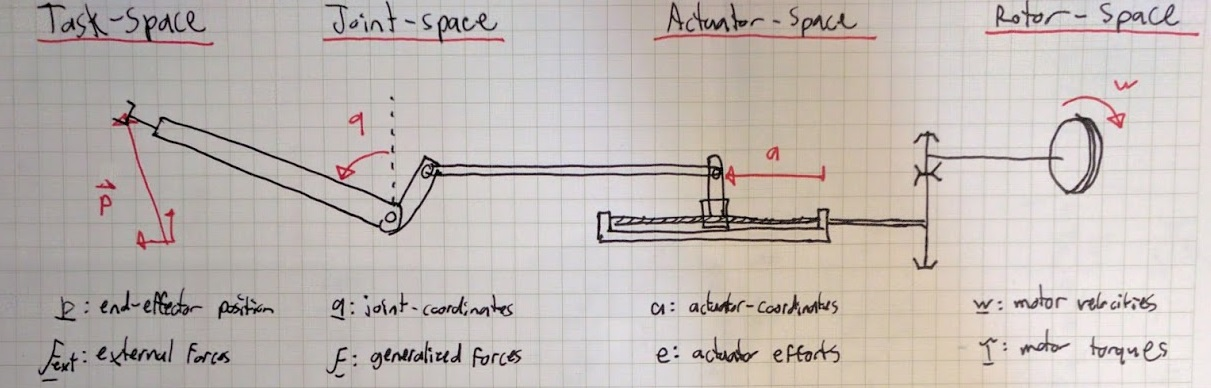
\includegraphics[width=0.99\textwidth]{coord.jpg}
	\caption{Coordinates system}
	\label{fig:coord}
\end{figure}

\begin{align}
\vec{\dot{p}}   &= J_e( \vec{q} ) \vec{\dot{q} }  \quad \text{ joint-space    --> end-effector   } \\
\vec{\dot{q}}   &= J_a( \vec{q} ) \vec{\dot{a} }  \quad \text{ actuator-space --> joint-space    } \\
\vec{\dot{a} }  &= R( \vec{q} )   \vec{ w      }  \quad \text{ rotor-space    --> actuator-space } 
\label{eq:coord_transform}
\end{align}


\begin{align}
H \vec{\ddot{q}} + C \vec{\dot{q}} + D \vec{\dot{q}} + \vec{g} =  \underbrace{ J_a^T(\vec{q}) R^T }_B  \vec{\tau} + J_e^T(\vec{q}) \vec{f}_e + J_c^T(\vec{q}) \vec{f}_c
\label{eq:manipulator}
\end{align}

\begin{align}
H   &= H_m + J_a^T R^T I_a R J_a        \\
C   &= C_m + J_a^T R^T I_a R \dot{J}_a  \\
D   &= D_m + J_a^T R^T B_a R J_a 
\label{eq:coord_transform}
\end{align}


\section{Contact}
\label{sec:contact}

\subsection{Constraints forces}
\label{sec:constraints}

\begin{align}
\phi( \vec{ q } ) = 0
\label{eq:constraint}
\end{align}

\begin{align}
\frac{d \phi( \vec{ q } ) }{dt} = J_c( \vec{ q } ) \vec{\dot{q}}  = 0
\label{eq:constraint_diff}
\end{align}

\begin{align}
\frac{d^2 \phi( \vec{ q } ) }{dt^2} = J_c( \vec{ q } ) \vec{\ddot{q}}  = 0
\label{eq:constraint_diff2}
\end{align}



\subsection{Impact forces}
\label{sec:impact}




